\chapter{Coordinación de Protecciones}

Este capítulo presenta el análisis de coordinación entre la protección principal del circuito 10-502 (relé AREVA MICOM P142 en SE Conucos) y las protecciones del proyecto AGPE en el nodo 3272966, con base en los ajustes oficiales entregados por ESSA y el perfil de demanda del alimentador.

\section{Ajustes del Relé de Cabecera}

\begin{table}[H]
    \centering
    \caption{Ajustes MICOM P142 --- bahía CTO 10502 (SE Conucos)}
    \begin{tabular}{ll}
    \toprule
    \textbf{Parámetro} & \textbf{Valor} \\
    \midrule
    Fabricante / modelo / serial & AREVA / MICOM P142 / 360 \\
    Tensión / RTC / RTP & 13,8 kV / 60 / 120 \\
    Funciones & 50, 50N, 51, 51N \\
    51 (fase) & 6 A sec $\rightarrow$ \textbf{360 A} prim; TMS 0,1; IEC VI \\
    50-1 (fase) & 36 A sec $\rightarrow$ \textbf{2160 A} prim; 0 s \\
    51N (tierra) & 2 A sec $\rightarrow$ \textbf{120 A} prim; TMS 0,15; IEC VI \\
    50N (tierra) & 20 A sec $\rightarrow$ \textbf{1200 A} prim \\
    Recierre 79 & 15/30 s; reset 60 s \\
    \bottomrule
    \end{tabular}
\end{table}

La curva IEC Very Inverse empleada es:

\begin{equation}
t = TMS \times \frac{13{,}5}{(I/I_s) - 1}
\end{equation}

\section{Demanda del Circuito vs Pickups}

El perfil horario de cabecera (19/03/2024) se contrastó con los pickups del relé:

\begin{table}[H]
    \centering
    \caption{Corrientes de demanda vs umbrales de protección}
    \begin{tabular}{lcc}
    \toprule
    \textbf{Magnitud} & \textbf{Valor} & \textbf{Observación} \\
    \midrule
    $I_{\max}$ cabecera (12:00) & 70,41 A & Demanda pico \\
    $I$ @ 09:00 / 15:00 & 61,05 / 68,55 A & Horas de estudio \\
    $I_{\min}$ cabecera (04:00) & 26,35 A & Valle \\
    Pickup 51 & 360 A & Margen $360/70{,}41 = 5{,}11$ \\
    Pickup 51N & 120 A & Margen $120/70{,}41 = 1{,}70$ \\
    $I_{\mathrm{gen}}$ referida a MT & 5,25 A & $\ll$ pickup 51 \\
    \bottomrule
    \end{tabular}
\end{table}

\begin{figure}[H]
    \centering
    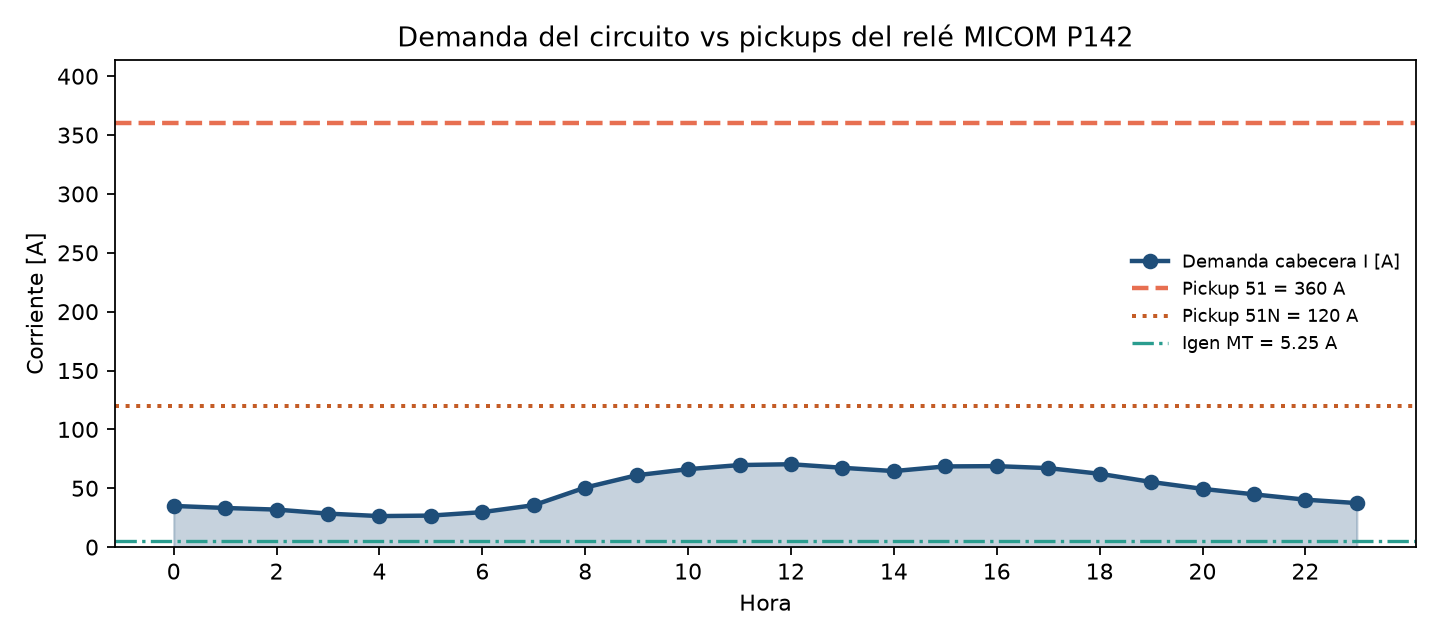
\includegraphics[width=0.95\textwidth]{figuras/fig_demanda_vs_pickup.png}
    \caption{Demanda horaria del circuito 10-502 vs pickups 51/51N e $I_{\mathrm{gen}}$ MT}
    \label{fig:dem_vs_pu}
\end{figure}

\textbf{Conclusión:} el pickup de fase está 5,11 veces por encima de la demanda máxima; la exportación del AGPE (5,25~A en MT) no opera el relé de cabecera.

\section{Protecciones del Proyecto AGPE}

\begin{table}[H]
    \centering
    \caption{Elementos de protección del lado BT}
    \begin{tabular}{lccc}
    \toprule
    \textbf{Elemento} & \textbf{Ajuste LV} & \textbf{Equiv. MT} & \textbf{Función} \\
    \midrule
    Breaker inversor (c/u) & 200 A & 3,33 A & Sobrecorriente equipo \\
    Breaker acometida & 400 A & 6,67 A & Seccionamiento POC BT \\
    Magnético acometida ($\approx 10\times$) & 4000 A & 66,7 A & Instantánea BT \\
    Inversor SOLIS & --- & --- & 27, 59, 81U/O, anti-isla \\
    \bottomrule
    \end{tabular}
\end{table}

\section{Curva Tiempo--Corriente (TCC)}

\begin{figure}[H]
    \centering
    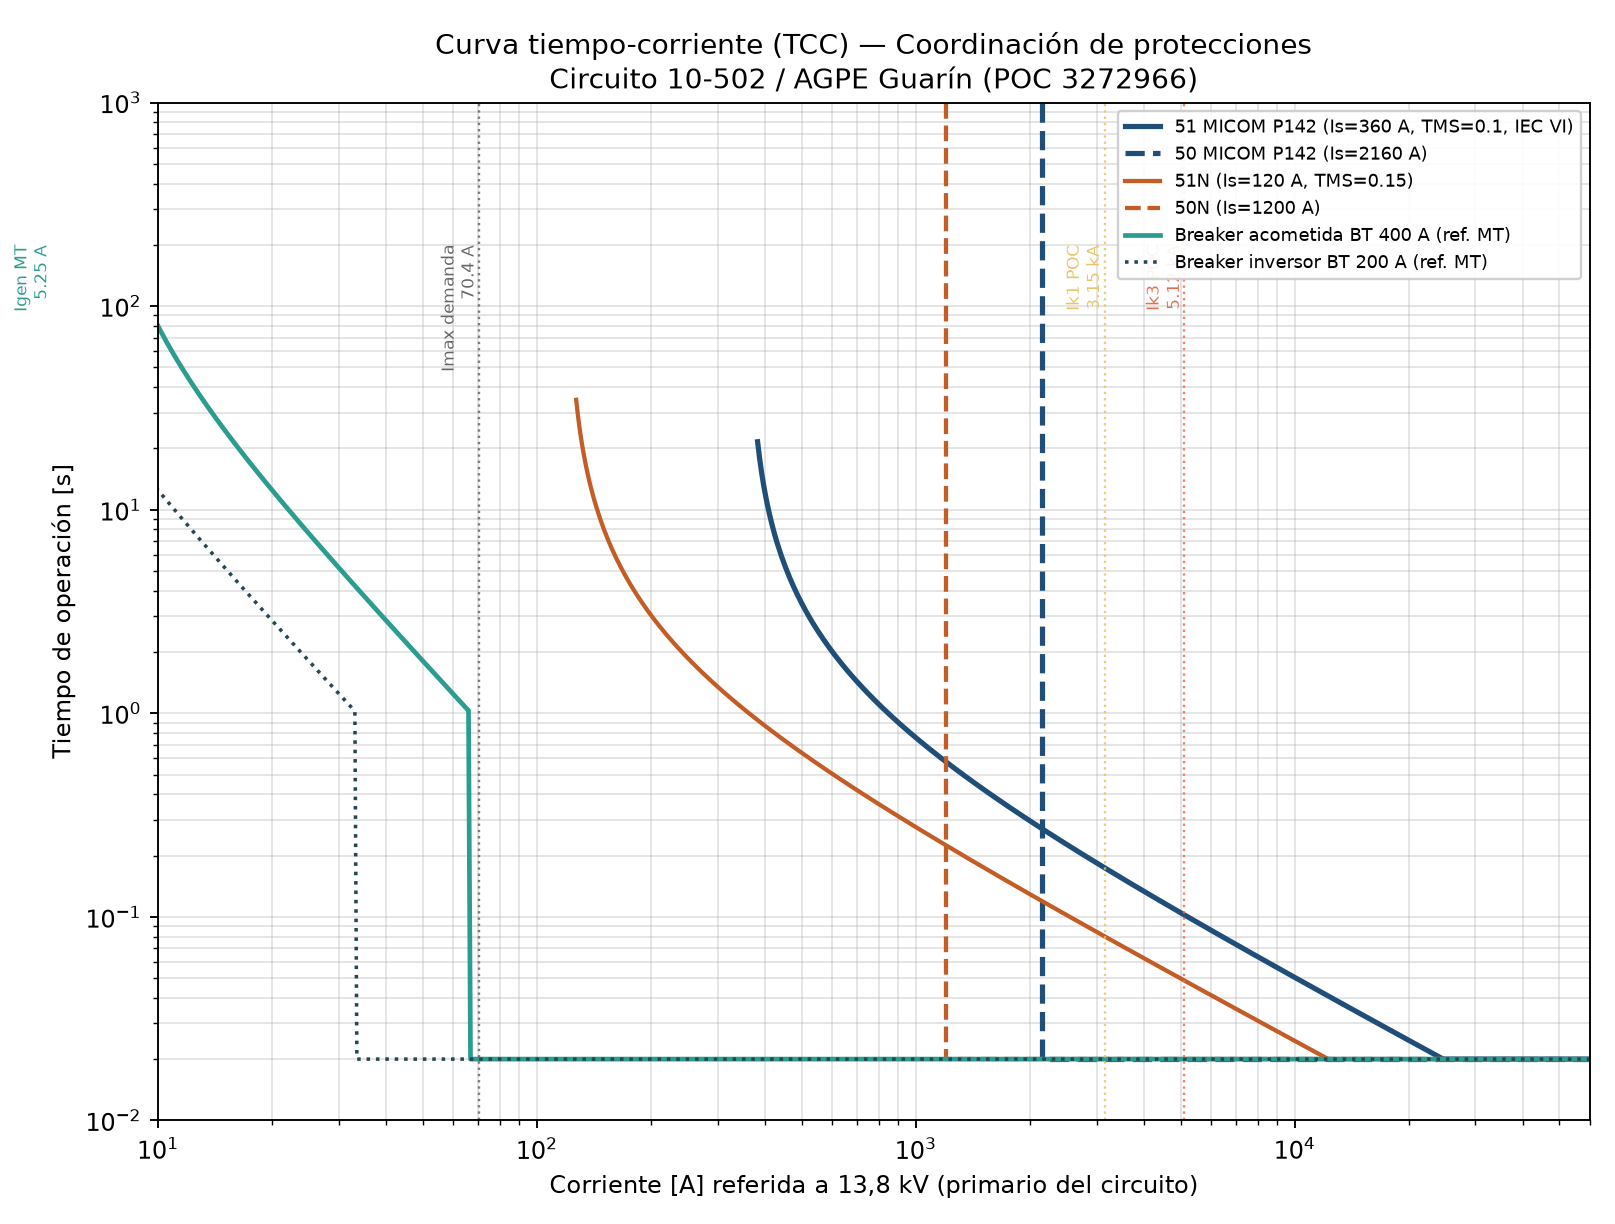
\includegraphics[width=0.98\textwidth]{figuras/fig_tcc_coordinacion.png}
    \caption{Curva TCC --- MICOM P142 (50/51/50N/51N) y breakers BT referidos a MT}
    \label{fig:tcc}
\end{figure}

\begin{table}[H]
    \centering
    \caption{Tiempos de operación de la función 51 (IEC VI, TMS $=0{,}1$, $I_s=360$~A)}
    \begin{tabular}{lccc}
    \toprule
    \textbf{Condición} & \textbf{$I$ [A]} & \textbf{$t_{51}$ [s]} & \textbf{¿Opera 50?} \\
    \midrule
    $I_{\max}$ demanda & 70,4 & No arranca & No \\
    $2\times I_s$ & 720 & 1,350 & No \\
    $5\times I_s$ & 1800 & 0,338 & No \\
    $10\times I_s$ & 3600 & 0,150 & Sí \\
    $I_{k3}$ en POC & 5120 & 0,102 & Sí \\
    $I_{k3}$ en SE & 27382 & 0,020 & Sí \\
    \bottomrule
    \end{tabular}
\end{table}

\section{Selectividad BT -- MT}

La impedancia del transformador de 150~kVA ($Z_{cc}=4{,}9\%$) limita la corriente de una falla en BT vista desde MT:

\begin{equation}
Z_t = 0{,}049 \times \frac{13{,}2^2}{0{,}15} = 56{,}92~\Omega
\quad\Rightarrow\quad
I_{k,\mathrm{thru}} \approx 133{,}9~\mathrm{A}
\end{equation}

Como $I_{k,\mathrm{thru}} = 133{,}9~\mathrm{A} < I_{51} = 360~\mathrm{A}$, el relé de cabecera \textbf{no arranca} ante fallas del lado BT. La selectividad es natural y total: solo operan los breakers del proyecto.

\begin{figure}[H]
    \centering
    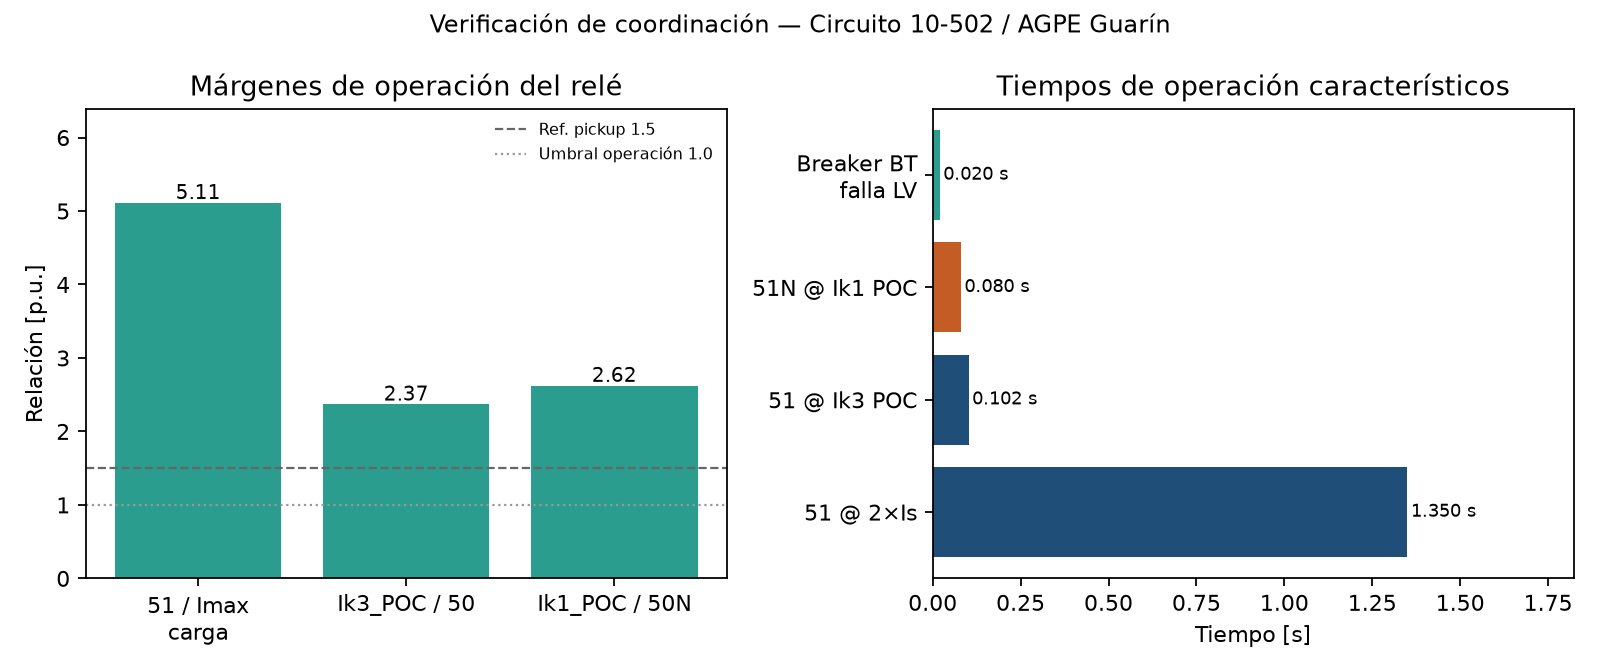
\includegraphics[width=0.95\textwidth]{figuras/fig_margenes_proteccion.png}
    \caption{Márgenes de pickup y tiempos característicos de operación}
    \label{fig:margenes_prot}
\end{figure}

\section{Respuesta ante Fallas en el POC (MT)}

\begin{itemize}
    \item Falla trifásica en 3272966 ($I_{k3}=5{,}12$~kA): supera el umbral 50 (2160~A) $\Rightarrow$ operación instantánea; $t_{51}\approx 0{,}10$~s como respaldo.
    \item Falla monofásica ($I_{k1}=3{,}15$~kA): supera 50N (1200~A); $t_{51N}\approx 0{,}08$~s.
    \item Aporte del SSFV al cortocircuito: $7{,}87$~A en MT ($0{,}15\%$ de $I_{k3}$ del POC) --- despreciable.
\end{itemize}

\section{Matriz de Cumplimiento}

\begin{table}[H]
    \centering
    \caption{Criterios de coordinación y resultado}
    \begin{tabular}{llc}
    \toprule
    \textbf{Criterio} & \textbf{Valor} & \textbf{Resultado} \\
    \midrule
    Pickup 51 $\geq 1{,}5\times I_{\max}$ & 5,11$\times$ & Cumple \\
    Exportación AGPE no dispara 51/50 & 5,25 A $\ll$ 360 A & Cumple \\
    Aporte CC SSFV $< 1\%$ & 0,15\% & Cumple \\
    Selectividad BT vs relé cabecera & $I_{k,\mathrm{thru}}<I_{51}$ & Cumple \\
    50/50N ven fallas MT en POC & Sí & Cumple \\
    Modificar ajustes MICOM P142 & --- & \textbf{No requerido} \\
    \bottomrule
    \end{tabular}
\end{table}

\section{Conclusión de Protecciones}

La coordinación entre el AGPE Guarín y el circuito 10-502 es satisfactoria. \textbf{No se requieren cambios} en los ajustes del relé AREVA MICOM P142. Se recomienda mantener los breakers BT en los rangos 140--200~A (inversor) y 350--500~A (acometida), y verificar en campo las funciones 27/59/81/anti-isla de los inversores SOLIS.
